\chapter{Validating state space screening calculations, a P3HT case study}
\label{chap:p3ht_validation}

The following chapter contains unpublished work written by me with guidance from Dr. Jankowski.

A Jupyter notebook demonstrating the tools mentioned in this chapter can be found in \autoref{app:p3ht_nb}, and a Zenodo dataset containing all data used in this chapter can be found at Ref.~\citet{Fothergill2022}.

\section{Introduction}

An important facet of applying molecular simulations to solve real-world engineering problems is ensuring that the simulations are correct.
While there exist general guidelines for improving simulation correctness (e.g., the TRUE principles \cite{Thompson2020}), specific instances will vary widely between disciplines because of individual workflows that govern scientific simulation pipelines. 
In this work we detail the application of TRUE principles for a common problem that arises in molecular simulations: performing molecular simulations across a set of thermodynamic state points to screen these conditions for structures of interest. 
Specifically, we consider a case study of validating structural predictions of the organic photovoltaic polymer P3HT. 

Organic photovoltaics (OPVs) are a focus of this research because they represent the best opportunity for cost-effective solar power.
The theoretical efficiency limit (Shockley-Queisser limit) for a p-n single junction solar cell is about 30\% \citep{Shockley1961}.
Multijunction cells may achieve efficiencies that surpass this limit, but they often do not have lower energy payback times as their production is more costly.
\autoref{nrel} shows the efficiency gains made by single junction silicon and organic photovoltaic devices over the last 30 years.
These are merely a selection among the many categories of PV devices.
The trend of the silicon cells shows that the efficiency gain is leveling off as the devices approach the Shockley-Queisser limit.
OPV devices, however, still have a lot of room for improvement, and recent increases in efficiency reflect this.
\begin{figure}[h!]
    \centering
    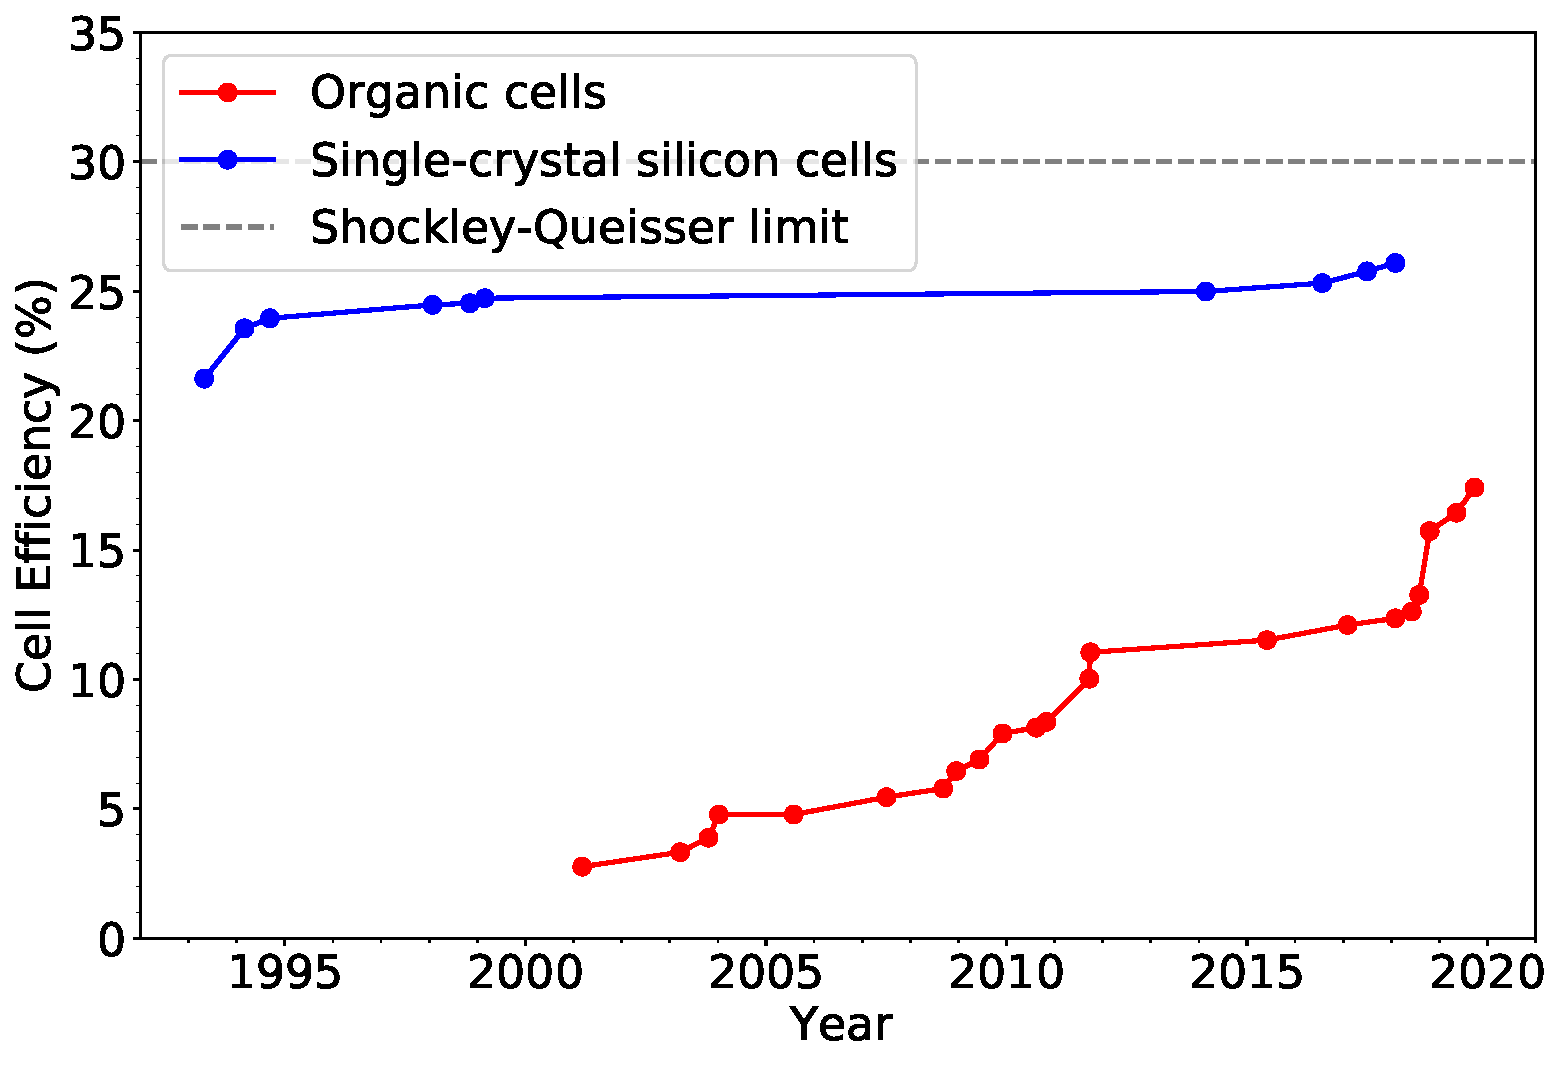
\includegraphics[width=0.8\linewidth]{figures/p3ht_val/NREL2020.pdf}
    \caption{Comparison of efficiencies in organic and silicon photovoltaic technologies from 1990 to present. The current state-of-the-art OPV, a mixed polymer, small molecule, and fullerene device, achieves 18.2\% efficiency \cite{Zhang2021}. Data taken from~\citet{NREL2020}.}\label{nrel}
\end{figure}
The potential of OPVs to achieve higher power conversion efficiencies depends on the morphology of the active layer. 
Molecular simulation can help to predict the combinations of donor and acceptor which will robustly self-assemble into a morphology best able to transport charge. 

A complication of the simulation of OPV polymers is that the properties which predict a device's efficiency, for example charge transport, span multiple length scales.
In order to model charge movement through a device, we need to know the position of individual atoms in order to discern the electronic environment and thus the likelihood of a charge hop, but we also need a bulk structure large enough that we can observe morphological features like the interdigitation of polymer lamellae to compare these morphologies to experiment.
But atomic resolution at length scales of hundreds of nanometers becomes computationally expensive, so simulating larger morphologies necessitates a simplified model.
By simplifying our model using coarse-graining techniques where multiple atoms are represented as a single bead we can more efficiently equilibrate larger length scales.
In additional to using a simplified model, the statepoint variables (including temperature, density, and solvent) must be carefully tuned to find the conditions under which the OPV morphology has the best self-assembly. 
Choosing a model and statepoint are some of the important choices a simulator must make when simulating OPV polymers. 
These choices should be informed by data, which increases the scope of this problem.
This chapter will discuss a previous work which laid the groundwork for making these choices using poly-3-hexylthiophene (P3HT), and the current work which aims to reproduce this work with improvements to the underlying tools which make them more transparent, reproducible, usable, and extensible (TRUE) \citep{Thompson2020}.

\section{Background} 

In previous work from our lab, Ref.~\citet{Miller2018}, hundreds of molecular dynamics simulations of P3HT polymer are performed across different temperatures, densities, and solvent qualities in order to ascertain at which statepoints the morphology would self-assemble into the most ordered structure.
%The temperatures and densities were chosen around the ranges used in experiment.
These hundreds of simulations at different statepoints were organized using custom python scripts which relied on creating and navigating a directory structure.
\begin{figure}[h!]
    \centering
    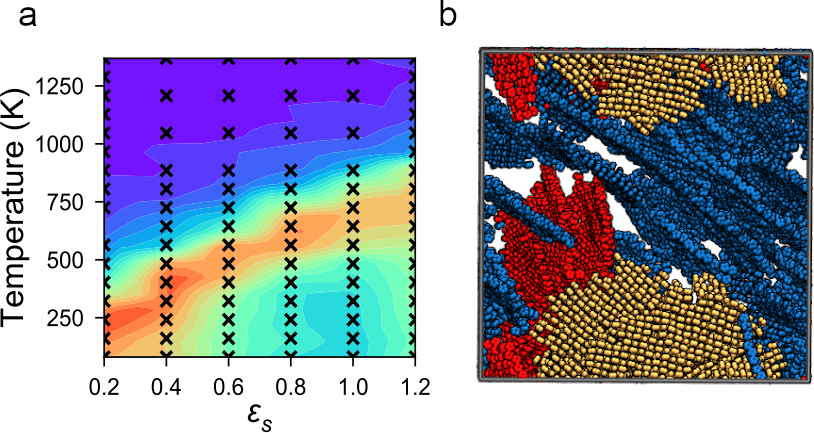
\includegraphics[width=0.8\linewidth]{figures/p3ht_val/miller2018_figs.png}
    \caption{(\textbf{a}) The degree of ordering, $\Psi$, at various temperatures and solvent parameters taken from Ref.~\citet{Miller2018}. (\textbf{b}) The three largest clusters (colored blue, red, and yellow in order of descending size) in a P3HT morphology taken from Ref.~\citet{Miller2018}.}\label{fig:miller18}
\end{figure}
\autoref{fig:miller18}a helps us to visualize the temperature and solvent parameter state space.
In order to aid the analysis of this state space, the order parameter ($\Psi$) was defined as the ratio of thiophene moeities in "large" clusters.
The clustering criteria takes into account the distance between thiophene centers and the angle between the planes of the thiophenes.
In \citet{Miller2018} the distance cutoff was 6 \AA, the angle cutoff was 20 $^{\circ}$, and a "large" cluster was defined as having 6 or more thiophenes.
\autoref{fig:miller18}b is a visualization of these clusters in a morphology.
The order parameter analysis required selecting specific atoms from the trajectory file based on their index.
The atom indices in this analysis were hard-coded for P3HT.
All the input files were made programmatically, so having hard-coded index values worked; however, if this analysis was to be used on polydisperse polymer lengths or a different molecule, it would have to be changed.
Simulated GIXS diffraction was used to compare the most highly ordered morphologies to experiment and they were found to show good agreement.
\citet{Miller2018} accomplished what they set out to do (validate a simplified model of P3HT) and performed work which was impressive in scope (hundreds of simulations!) and all the code is freely available to all, but how can we redesign these tools to be easier to use for the next molecule and the next user?

%% transition here from Evan's work to mine
To reproduce the work of \citet{Miller2018}, this workflow must be designed to handle a broad computational scope.
It must be able to create and manage a large parameter space, move data between multiple different pieces of code, translate units, and perform analysis on selected particles from simulation trajectories.
Much of my work in the lab has been to design tools which makes these tasks more transferable, reproducible, usable, and extensible (TRUE) \citep{Thompson2020}.
Transferable means the code is general enough to be used in different ways or applied to different problems.
Reproducible means enough information is provided that the work can be redone and no important details regarding the process are obscured.
Useable by others means that other people---especially people outside your circle---can actually use this tool. This entails that not only is the source code is freely available and easy to install but also that users can understand how to use it without too much cognitive overhead. This can be helped with permissive, open licensing, dependency documentation and packaging (including containers), and thorough documentation and examples.
Extensible mean that others can build upon the work you have done.
If this project is going to have the desired impact (i.e., using molecular simulation to identify novel OPVs), every step of the process and the resulting data must be straightforward to reproduce and validate.
The nature of a multiscale simulation requires translation between formats and units and accurate handling of large data, and thus requires infrastructure to reduce error.
Although the molecular and computational scope of this project is broad, by using and building upon existing architectures and adhering to recent guidelines in the computational sciences community we can manage the multiscale nature of this project and contribute to reproducible science.
This chapter will demonstrate that we can reproduce and validate our P3HT morphologies while using MoSDeF tools to help our methods to be more TRUE.

\section{Statement of Need}

In order to sample the parameter space, we need to be able to spin up a large number of simulations (i.e., initializing our simulation volume, implementing the model, and running the simulation) and accurately access each simulation output to perform analysis.
The order parameter analysis involves selecting the atoms that are part of a chemical moiety and calculating the distance and angle between each potential neighbor moiety. 
If the potential neighbor meets the clustering criteria, it is added to the cluster.
The order parameter can then be calculated as the ratio of the number of the moiety in large clusters vs the total number in the morphology.
And the GIXS analysis involves converting the simulation trajectory to the format required by the diffractometer package including unit conversion.

Before we address challenges in the implementation, it is important to note how we solved issues related to installing the software stack.
Often this step goes unmentioned, but installation of software packages and managing dependencies can be a huge hurdle for computational scientists. 
To prevent this, we have built pipelines for all our code repositories (using GitHub Actions) which automatically build docker containers from each tagged version of the repository and the latest master branch. 
These containers can be used with the docker or singularity applications and contain the exact code state present in the repository along with static versions of its dependencies.
This allows our software to be used without ever having to manually install it or manage its dependencies. 
Not only does this make our software stack easier to use, but it makes it more portable---we can have the exact same environment on our school cluster or XSEDE.
And if someone wants to reproduce our work, they can access the exact container we used.

The first challenge, managing a large dataspace, is handled using the Signac framework. Although designing code to work within a framework like Signac does add some cognitive load, after this initial lift the project becomes more extensible and flexible regrading changes in the parameter space. We will cover the tool designed to manage and submit OPV MD simulations within this framework, PlanckTon, later in the chapter.

Although the application of the united-atom model to our P3HT system was not overly complicated as it only contained 3 types, it required manual atom typing, which presented another hurdle to applying this method to a new and perhaps more complicated compound. 
By using the foyer forcefield dissemination and atom-type engine \cite{foyer} our atom types can be automatically assigned based on the chemical connectivity. This allows us to more easily extend to new compounds.

Calculating the order parameter originally depended on a workflow that was hard-coded for P3HT and selected specific atom indices---this depended on the particle order in the simulation being the same every time, which it was because routine initialization methods were used, but it did not allow for the method to be applied to other compounds.

\section{Tools}

Next we will discuss the various tools used in this project.  \autoref{fig:p3ht-workflow} gives an overview of how these tools work together to perform the structural analysis.
\begin{figure}[h!]
    \centering
    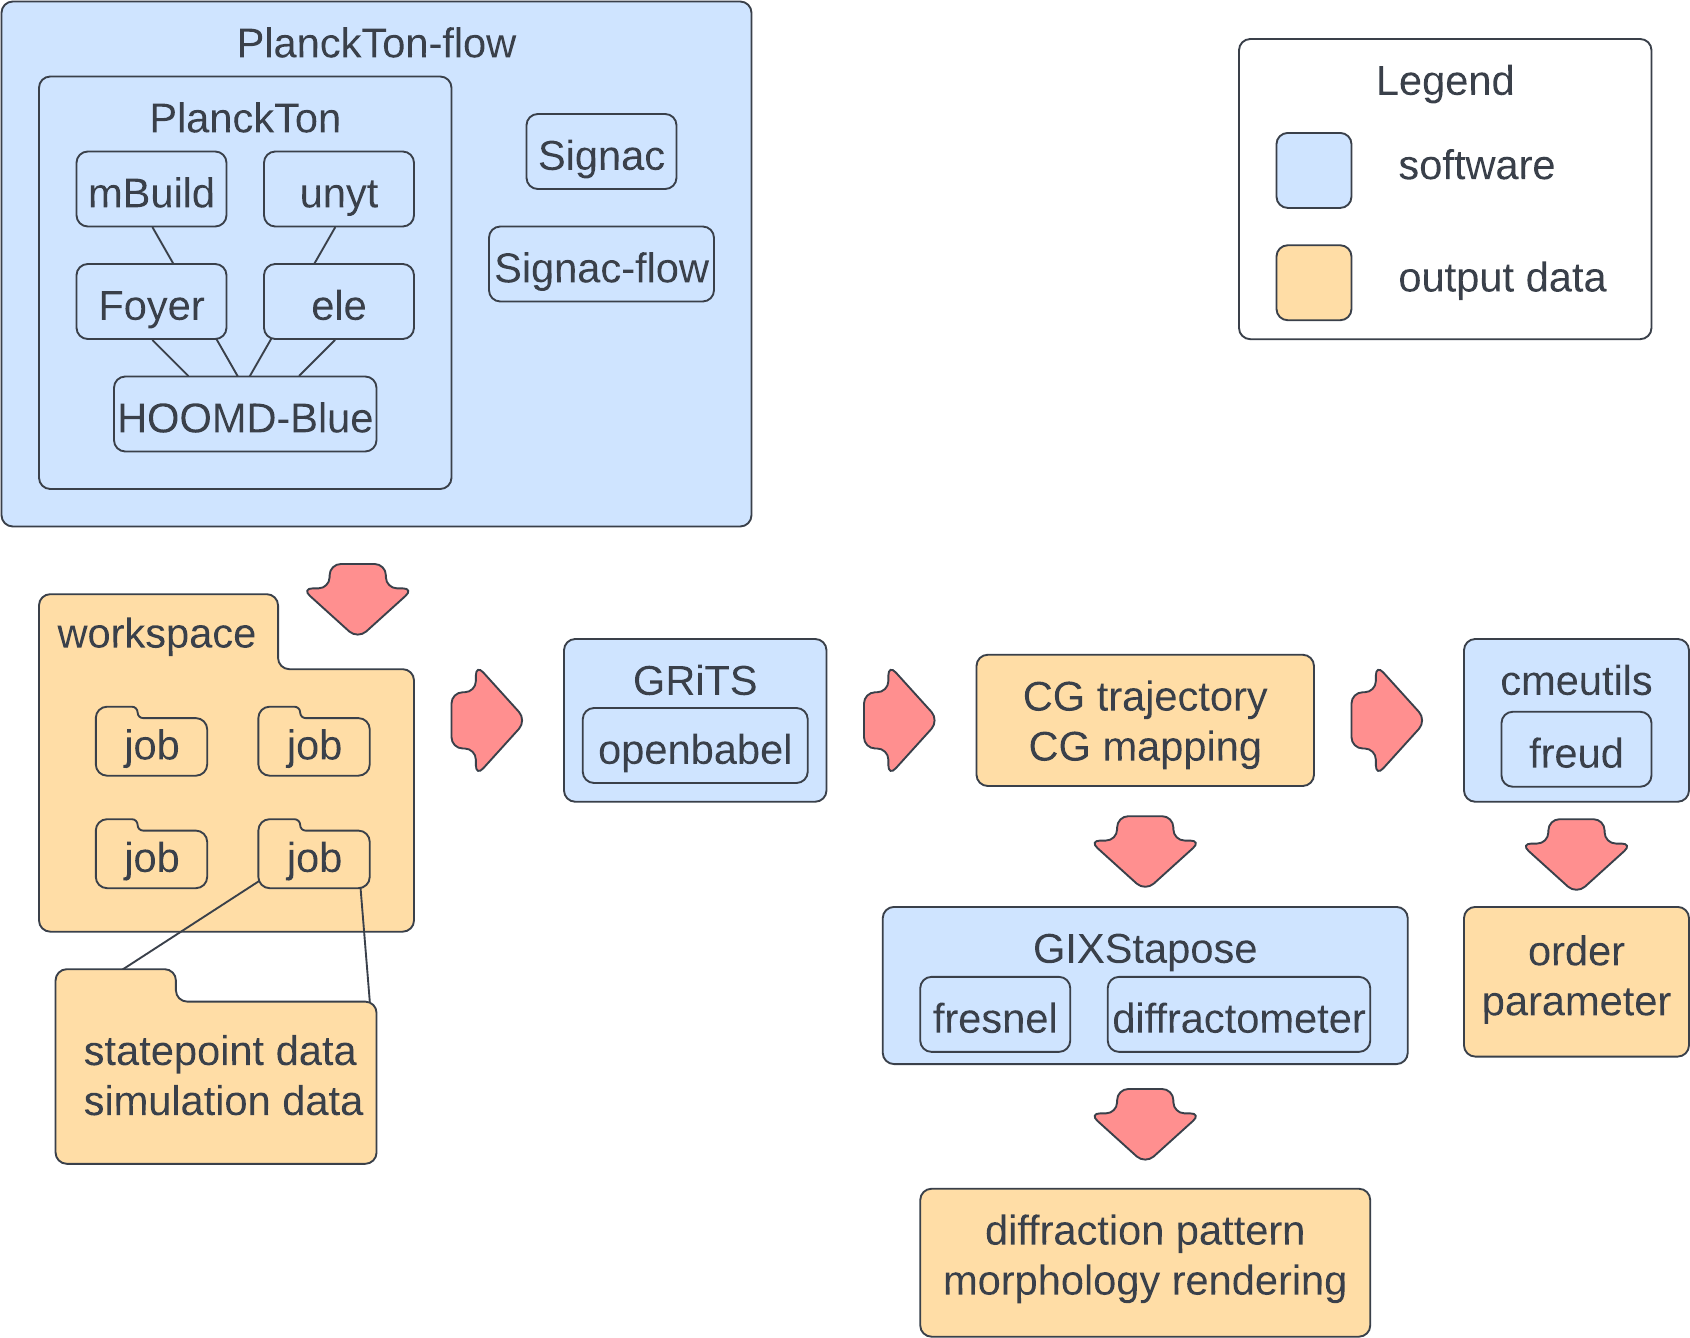
\includegraphics[width=0.8\linewidth]{figures/p3ht_val/workflow.png}
    \caption{Overview of the structural analysis workflow. First, the workspace is created in the PlanckTon-flow framework and all simulations are run. Then GRiTS is used on the output simulation data to find the thiophene centers. Finally, the order parameter function in cmeutils is used to calculate the order parameter of each simulation trajectory and GIXStapose is used to perform GIXS analysis.}\label{fig:p3ht-workflow}
\end{figure}
This workflow was designed such that the output from each code can be used as the input for the next with little to no modification. 
Many of these code bases are collaborative works, so I will give credit to the contributors and creators of the underlying building blocks.

\subsection{PlanckTon}
In order to initialize simulations in a reproducible way, we have designed PlanckTon: a wrapper for the initialization, management, and submission of organic photovoltaic molecular dynamics simulations using the HOOMD-Blue engine \citep{planckton, Jankowski2019, Anderson2020}.
The PlanckTon software includes some OPV compounds commonly used in our lab to guarantee that all simulations are initialized with the exact same starting compound; however, the workflow is designed to easily accept any MoSDeF compatible chemical input file format including SMILES strings. 
The code base also ships with custom XMLs for OPLS-UA and GAFF and a separately packaged GAFF XML \citep{DeFever}, but is compatible with any Foyer XML. 
The initialization procedure of PlanckTon is as follows: First the user selects a compound or mixture of compounds, the number of said compounds, the temperature, the density, and the solvent parameter. 
As in Ref.~\citet{Miller2018}, the solvent in PlanckTon is modelled implicitly, so the solvent quality, $\epsilon_{s}$, refers to a scaling factor on the non bonded forces.
In order to more robustly achieve high density morphologies, the simulation volume is initialized at a lower density and then shrunk down to the desired density at high temperature\cite{Jankowski2013,Marsh2014,Jones2017,Henry2017a,Miller2018}. 
The creation of our simulation volume, the forcefield atom-type assignment, and the creation of the HOOMD force objects is completely handled by mBuild and foyer in the MoSDeF framework\citep{mbuild,foyer}.
By using the modular, general system initialization of the mBuild and foyer, we get two benefits: (1) we draw on the knowledge base of the MoSDeF community--more users means we can find and resolve errors more quickly, and (2) we can more easily incorporate the system initialization in our other projects. 
Once the system and forces are initialized, PlanckTon uses the NVT ensemble via the Nosé-Hoover thermostat \citep{Martyna1994d, Martyna1996} as implemented in the HOOMD-Blue molecular dynamics engine. 
The initial velocities and angular momenta are randomly assigned from the Maxwell-Boltzmann distribution.
By having our entire process scripted, we can have everything about our process documented and available for scrutiny and reduce the potential human error inherent when switching between codes or transferring files.
Through PlanckTon-flow, this tool is supported by the Signac framework, which handles the parameter space initialization and management and submission to various computing clusters. Because this workspace is created using Signac, Signac can be used to navigate it. This allows to reference our data via the statepoint (e.g., what temperature and $\epsilon_{s}$ it was run at) without ever having to create or manage a complicated directory structure or naming scheme.

PlanckTon was started by my lab mates Mike, Evan, and Matty, and I have assumed responsibility for its development including:
Updating to HOOMD 2 allowed us to use the HOOMD simulation initialization functions in mBuild. This allows the package to be more modular and useable by others; any improvements or bugfixes needed in the \lstinline{create_hoomd_simulation} function can be contributed back to mBuild, which allows the whole community to benefit.
Adding automated docker container builds.
Generalizing the initialization procedure to allow starting compounds to be loaded from SMILES strings or any input file and these untyped compounds can be typed on the fly using any foyer compatible forcefield.
Adding support for all HOOMD neighborlists, which allows better sampling of sparse systems. 
And adding support for user specified temperature ramps, allowing users to perform temperature annealing, a technique used in OPV active layer synthesis.
In order to be more clear about the units used in PlanckTon, the unyt package is used to handle all unit conversions. This package allows for values to be tagged with their unit and then all conversions can be handled by the package.

PlanckTon is unique, but there exist other tools to manage molecular dynamics simulations. There is a web-based application that facilitates MD simulation using cloud computing services and automates related tasks \citep{Nicolas-Barreales2021} and a command line tool that automates many common MD tasks \citep{Rackers2018}, but I have not seen a pure python implementation which can also manage a large dataspace.

\subsection{GRiTS}
I developed GRiTS as a tool to assist in applying a coarse-grain mapping and to backmap a coarse-grain system to a fine one. 
Although the fine-graining capabilities are still under development, the coarse-graining is robust enough to apply a mapping to an entire system trajectory. 
This mapping can also be used to pick out specific chemical moieties from a morphology. 
GRiTS works using SMARTS matching---implemented in OpenBabel---to map atomic indexes to coarse grain beads. 
Once all the atomic indices are assigned to a bead, then bonds are inferred between coarse-grain beads based on the atomistic bonding scheme. 
For example, if an atom in bead A is bonded to an atom in bead B, beads A and B are assumed to be bonded. 
When looking at an entire simulation trajectory, the SMARTS matching algorithm can be prohibitively expensive.
So GRiTS uses the following simplifying assumptions: Chemical bonds are not formed or broken over the course of the simulation---this allows only the first frame of the trajectory to be used for mapping. 
Using only the first frame of the trajectory is also useful because this way the molecules in the system can be guaranteed to be chemically reasonable---i.e., the bonds and angles are not distorted, aromatic systems should be planar, etc. 
It is also assumed that if molecules have the same number of atoms, they have the same chemical structure. 
This allows us to use the clustering algorithms of implemented in the Freud analysis library to break the snapshot into molecules and only perform SMARTS matching on each molecule type, then extrapolate the mapping out to other molecules of the same type.

When working with a UA system, GRiTS can also infer hydrogen positions and bonding. This allows for SMARTS strings to find matches in UA systems. The hydrogen inferring method uses OpenBabel and requires that the first frame of the trajectory be chemically reasonable.

There are other tools which handle creating coarse-grain mappings such as VOTCA \citep{Ruhle2009}. 
This tool will crate a coarse grain trajectory from an atomistic one given an XML file mapping which requires the user to specify everything from the atom types involved in the bead to the bond and angle information.
VOTCA also has many other functions that GRiTS does not such as coarse-graining (including potential development), charge-transport, and excitation transport.
VOTCA requires the user to edit an xml file in which formatting and whitespace have meaning, and define not only the mapping but also the bonding and angles for the coarse grain mapping, which could easily be inferred from the mapping scheme.
Creating a mapping with GRiTS is more intuitive because the only parameter needed is a SMILES string, there are no potentially difficult to parse files for the user to edit, and all bonding and angles within the coarse grain structure are inferred.

\subsection{GIXStapose}
GIXStapose is a package which allows users to connect the real space view of a chemical structure to its simulated grazing incidence X-ray scattering (GIXS) pattern. (The name ``GIXStapose'' is a portmanteau of ``GIXS'' and ``juxtapose.'') 
I developed GIXStapose as wrapper for the diffractometer package and the fresnel ray tracing library \cite{Diffract, Jones2017, fresnel}
GIXStapose works by translating the structural information in many chemical input files into the formats needed by these two packages, and in the process can link rotations of the real space image to its diffraction pattern. 
The camera information used to generate the real space rendering and the diffraction pattern can be accessed and saved, allowing users to recreate the exact figure.
The package has an interactive graphical user interface (GUI), but is completely modular and can be run in a scripted fashion to generate reproducible figures and diffraction patterns along with translation of units. 
This work was presented at Scipy2020 \cite{gixstapose-scipy}. 

\section{Methods}
\subsection{Generate simulation data}
A PlanckTon-flow workspace of 40 simulations defined by their temperature and solvent parameter ($\epsilon_{s}$) was initialized. Each system comprised of 100 united-atom (UA) P3HT 16-mers parameterized with GAFF. %(The compound can be found in planckton as "P3HT-16-gaff" and the forcefield is "gaff-custom".) 
All nonbonded forces used a cutoff value of 8.91 \AA~ (2.5 times the largest sigma value). The target density for all was 0.56 $\frac{g}{cm^{3}}$. All simulations used a timestep of 2 fs and started by shrinking the box from 125 times the the target volume to the target volume (789 nm$^3$) at 629 K, with a thermostat coupling value (tau) of 2 ps, run over 0.2 ns. Once the shrink step was finished, each simulation was run at its own combination of temperature and $\epsilon_{s}$ ranging from 125, 188 to 629 K and 0.2 to 1.0, respectively. These runs used a thermostat coupling value (tau) of 0.6 ps and were run for 200 ns. All were run in the \lstinline{cmelab/planckton_gpu:v0.6.1} docker container.

\subsection{Create coarse grain mapping}
The GRiTS \lstinline{CG_System} class was used to find indices of atoms in thiophenes using SMARTS string ``c1cscc1'' and inferred hydrogens. This created a new coarse-grain trajectory file with beads at thiophene centers and a json file which contains the SMARTS string which generates the mapping and the atom indices in the atomistic trajectory as a key value pair.

\subsection{Calculate order parameter}
The \lstinline{order_parameter} function in cmeutils was designed to use the coarse grain trajectory and the mapping to calculate the average order parameter of the last ten frames of the trajectory. An angle cutoff 10 $^{\circ}$ and a distance cutoff of 6 \AA~ was used as the clustering criteria.

\section{Results and Discussion}

With the updates made to this workflow, first let's check that we get quantitatively similar results.
\begin{figure}
    \centering
    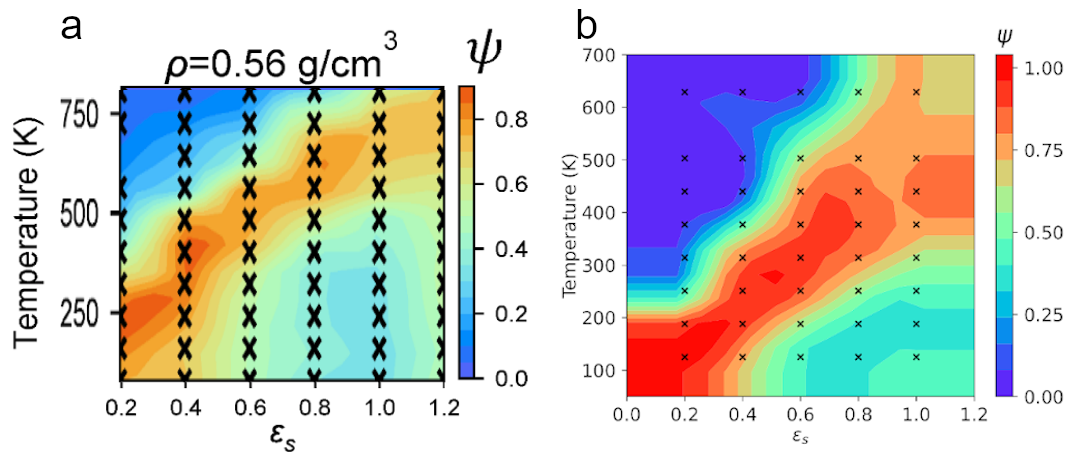
\includegraphics[width=0.8\linewidth]{figures/p3ht_val/Miller2018_fig3comparison.png}
    \caption{The degree of ordering, $\psi$, of P3HT at various solvent qualities, $\epsilon_{s}$, and temperatures. Red regions denote high order, blue regions are disordered. Each black "x" indicates a measurement, values between are interpolated. Part a is taken from \citet[Figure 3a]{Miller2018} and has been cropped and scaled to focus on the region of interest and make the plot bounds closer in value. Part b was created using the order parameter value from each simulation trajectory and the RectBivariateSpline interpolation function from the Scipy library. The final z values were adjusted such that no order parameter was greater than 1 or less than 0.}\label{fig:order}
\end{figure}
\autoref{fig:order} shows good qualitative agreement between the previous findings of \citet{Miller2018} and the order parameter trends found in this work. The absolute value of the order parameters seen in this work are, in general, higher than those observed by \citet{Miller2018}. This may be due to the initial high temperature shrink period used in this work which is similar to Protocol 2 in \citet{Miller2018} which was shown to achieve faster equilibration and more robust ordering.

Next the high order regions were further examined using GIXS analysis (see \autoref{fig:highorder-dp}).
\begin{figure}
    \centering
    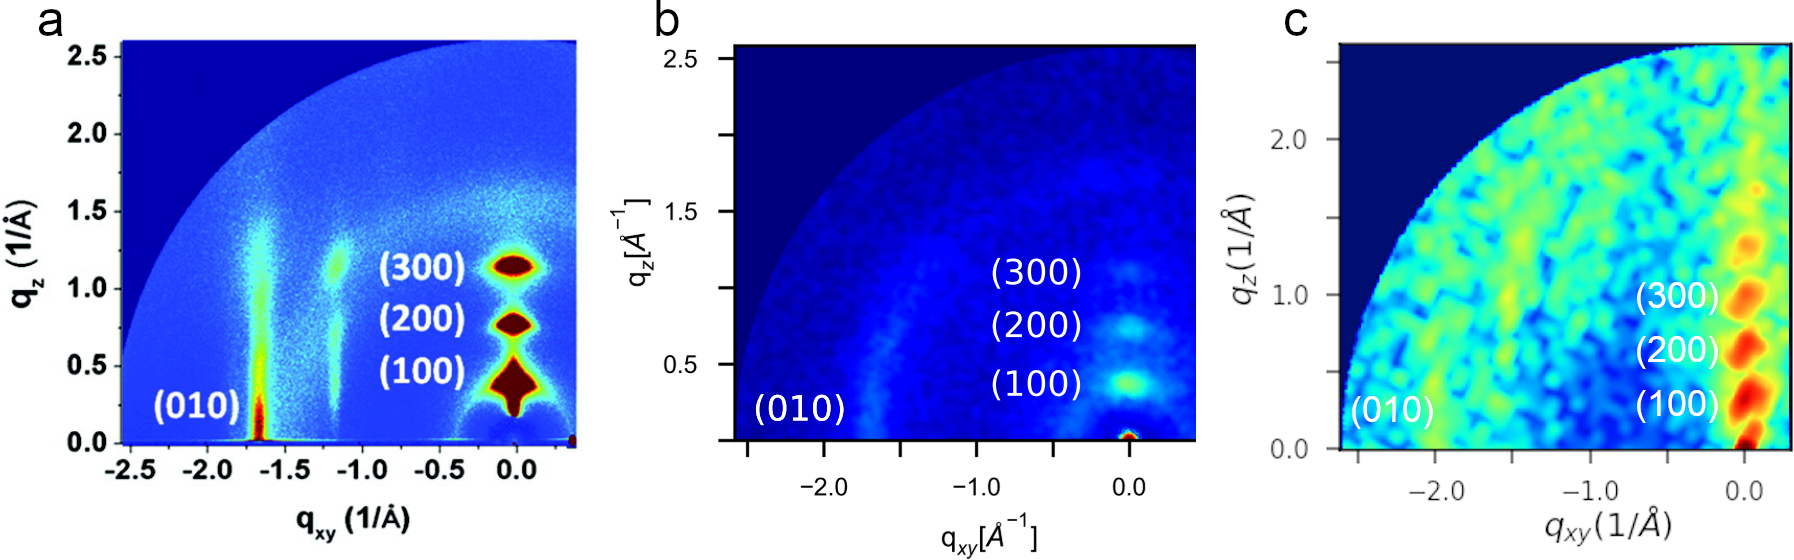
\includegraphics[width=0.8\linewidth]{figures/p3ht_val/Miller2018_fig6comparison.png}
    \caption{Diffraction patterns of P3HT from (a) experimental GIXS of neat P3HT \cite{Ko2012}, (b) simulated GIXS \citep{Miller2018}, and (c) this work. Part c was generated in GIXStapose using thiophene centers found using GRiTS from the simulation trajectory ran at $\epsilon_{s}$ 0.4 and T 251K.}\label{fig:highorder-dp}
\end{figure}
\autoref{fig:highorder-dp} shows good quantitative agreement between this work, experiment, and previous work. This also shows that high order parameter is a good predictor of clear GIXS peaks.
The GIXS data in \autoref{fig:highorder-dp}c is noisier because was generated using a very small system (1,600 points vs 15,000 points in part b). However, even in spite of this, it is clear that qualitatively the same structural features seen in previous works and experiment are present. 
And we can check that the real space distances these peaks correspond to are reasonable using the following equation
\begin{equation}\label{eq:peaks_to_dspace}
    d_{real} = \frac{2 \pi}{d_{peak}}
\end{equation}
where $d_{peak}$ is the distance of the bright spot from the origin.
The (100) peak corresponds to a periodic distance of 16.4 \AA~ and and the (010) peak to a distance of 3.50 \AA; \citet{Duong2013} report a lamellar spacing of 16.5 \AA~ and a pi-stacking spacing of 3.83 \AA~ for neat P3HT. 
There is room for users to choose multiple points within a large, smeary peak such as shown in \autoref{fig:highorder-dp}c, so these values are reasonable but could vary depending on the user's choice.

Using all particles in the united-atom thiophene may result in easier to see spots in the diffraction pattern (see \autoref{fig:ua-vs-cg-dp}).
\begin{figure}
    \centering
    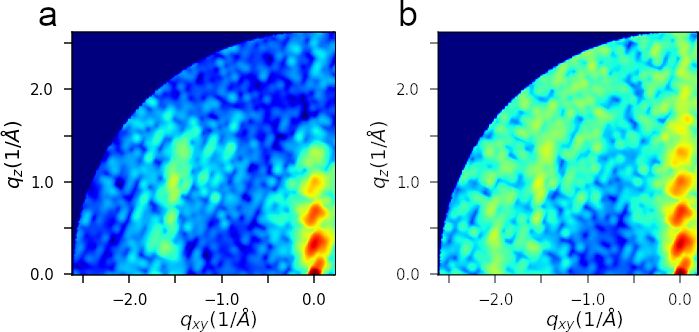
\includegraphics[width=0.8\linewidth]{figures/p3ht_val/ua_vs_cg_dp.png}
    \caption{Diffraction patterns of P3HT using (\textbf{a}) all thiophene particles in the UA trajectory (\textbf{b}) thiophene centers found using GRiTS. Both patterns were generated using GIXStapose at the same camera angle on the simulation trajectory ran at $\epsilon_{s}$ 0.4 and T 251K.}\label{fig:ua-vs-cg-dp}
\end{figure}
Although coarse-graining may provide clarity with much larger or less ordered structures, in this very small ordered system, the peaks are more easily visible in the when all the thiophene particles are used in diffraction.

As \autoref{fig:highorder-dp}c was generated using GIXStapose, we can examine the real space structure from the exact viewing angle the diffraction pattern was generated from. 
\begin{figure}
    \centering
    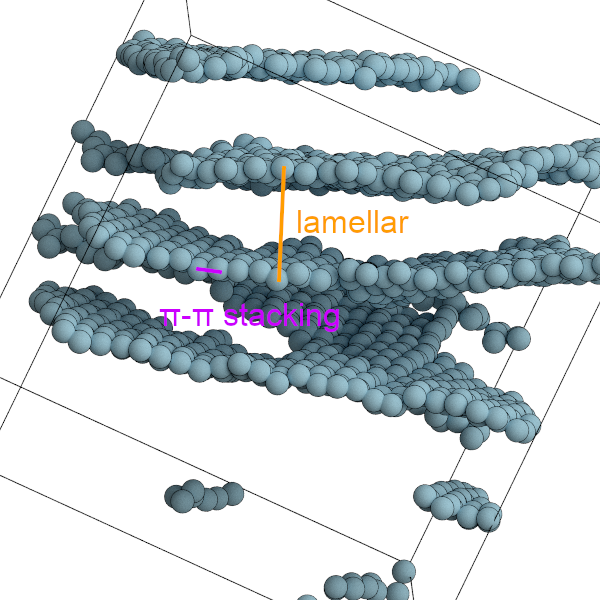
\includegraphics[width=0.8\linewidth]{figures/p3ht_val/scene_annotated.png}
    \caption{Real space structure of thiophene centers found using GRiTS from the simulation trajectory ran at $\epsilon_{s}$ 0.4 and T 251K. This figure is generated using fresnel via GIXStapose with the same "camera angle" as \autoref{fig:highorder-dp}c. }\label{fig:highorder-centers}
\end{figure}
\autoref{fig:highorder-centers} shows the thiophene centers at a high-order statepoint. We can clearly see the lamellar spacing in the vertical direction, and less clearly the $\pi$-$\pi$ stacking in the horizontal direction. By viewing the real space structure from the exact angle as the diffraction pattern, it is easier to correlate periodic features with their diffraction peaks.

To confirm that the thiophene center beads are being placed correctly, we can view an overlay of the thiophene centers with a frame of the unaltered UA simulation trajectory.
\begin{figure}
    \centering
    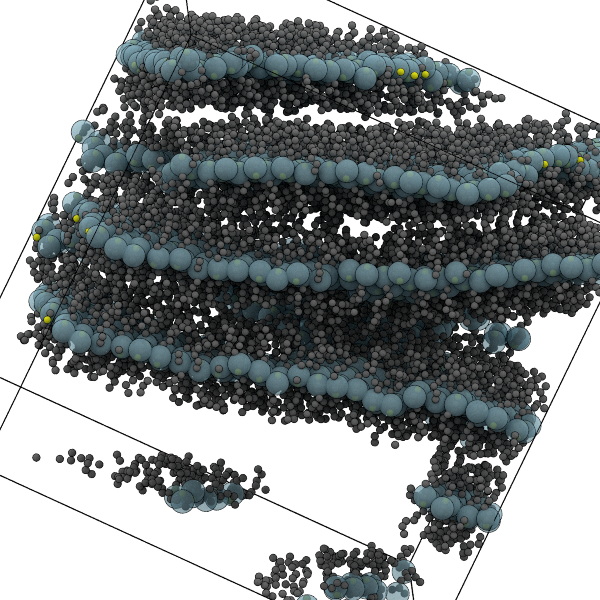
\includegraphics[width=0.8\linewidth]{figures/p3ht_val/cg-overlay_scene.png}
    \caption{Overlay of thiophene bead centers (translucent blue) found using GRiTS with united atom carbon (grey) and sulfur (yellow) in P3HT simulation trajectory ran at $\epsilon_{s}$ 0.4 and T 251K. This figure is generated using fresnel via GIXStapose with the same "camera angle" as \autoref{fig:highorder-dp}c and \autoref{fig:highorder-centers}}\label{fig:centers-overlay}
\end{figure}
\autoref{fig:centers-overlay} shows that the thiophene beads are correctly capturing the geometric centers of the thiophene moieties in the trajectory given that the sulfur atoms are found almost entirely within the thiophene beads. This view also gives us a better perspective on what forces may be causing the lamellar separation---namely, side-chain interactions.

We can also show correlation between low order parameter and disordered systems with no GIXS peaks (see \autoref{fig:loworder-centers} and \autoref{fig:loworder-dp}).
\begin{figure}
    \centering
    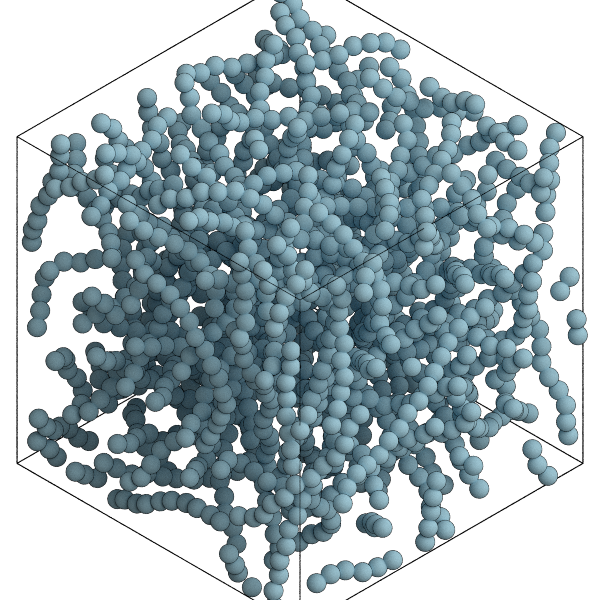
\includegraphics[width=0.8\linewidth]{figures/p3ht_val/cg-trajectory-amorphous_scene.png}
    \caption{Real space structure of thiophene centers found using GRiTS from the simulation trajectory ran at $\epsilon_{s}$ 0.2 and T 629K. This figure is generated using fresnel via GIXStapose with the same "camera angle" as \autoref{fig:loworder-dp}c}\label{fig:loworder-centers}
\end{figure}
\begin{figure}
    \centering
    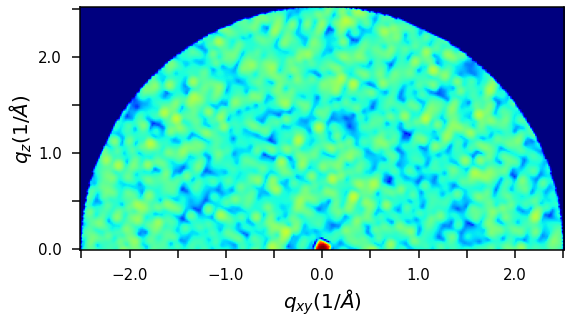
\includegraphics[width=0.8\linewidth]{figures/opa_notebook/Order_parameter_analysis_21_0.png}
    \caption{GIXS pattern generated in GIXStapose using thiophene centers found using GRiTS from the simulation trajectory ran at $\epsilon_{s}$ 0.2 and T 629K.}\label{fig:loworder-dp}
\end{figure}
\autoref{fig:loworder-centers} shows the thiophene centers in a basically random configuration and \autoref{fig:loworder-dp} shows a general lack of peaks.

So, we have demonstrated that our ordering trends observed in P3HT are robust to changes in the forcefield (OPLS-UA to GAFF-UA). And that the changes to simulation initialization (more incorporation of MoSDeF tools) and analysis (using GRiTS to detect thiophenes) have not skewed our results. Next let's discuss the potential effect of our TRUE changes.

\section{Conclusions}

By using  mBuild with foyer in PlanckTon to initialize our simulations, we can more easily use different input file formats including smiles strings and any foyer forcefield. 
Using GRiTS to select the desired part of the molecule removes any need for manual indexing, which allows us to more easily extend the order parameter calculation to other planar, conjugated molecules like perylene or ITIC.
Working within the Signac framework allows us to quickly and easily sample the necessary parameter space without needing to manually create or manage directories. 
We've also implemented semantic versioning in all our lab's codebases with version tagged docker containers which helps users to keep track of when changes are made and ensure we use the same code state.
By using and building on existing code, we work with a community of open-source molecular simulators. 

The ultimate success of this project to me is if someone else can use it. 
And in order to achieve that goal, I have tried to develop code with the next user in mind.
I know it can be daunting to be handed someone else code. 
If the only way to learn how to use it is to read through the code comments (or just the code itself) and try to figure it out, users may prefer to simply write their own. 
Even when good user documentation is provided, often these bespoke codebases have specific dependencies which may not be continuously maintained so they break in updated installations.
We can consider the effort put in to providing containers with the complete functioning software stack and writing thoughtful user documentation and examples as a force multiplier. 
If the goal of a scientific codebase is to accomplish work, then the more people who can use this code, the better.
Also writing our code to be more modular and general can help it to apply to more situations. 
For example the GRiTS code was designed to create coarse-grain mappings, but the mappings can also be used to find instances of a SMILES pattern with a trajectory as was done in this study.

It is hard to measure the success of that goal, but I submit the following examples:
In the summer of 2021, our lab hosted two students from the NSF Research Experience for Undergrads (REU) program and a high school teacher from the Research Experience for Teachers (RET) program. 
None of these students had any prior knowledge of shell scripting, python, or molecular simulation. 
After a week or so of introductory training, the three researchers were introduced to PlanckTon. 
Each researcher chose a molecule, and together with three undergrad researchers in the lab, were able to run 24K SUs worth of MD simulations on XSEDE using PlanckTon. 
A new PhD student in our lab with a strong background in software engineering but new to molecular simulation and chemistry was able to use GRiTS to create a coarse grain mapping in a matter of days. 
She did this without any one-on-one training beyond the documentation and examples.

By developing code with TRUE principles, other scientists can more easily use and extend this project.
Hopefully this software ecosystem will continue to be dynamic and evolving. 
The work of \citet{Miller2018a} has shown the importance of polydisperse polymer lengths and their ability to form tie-chains for charge transport simulations. 
Tools for initializing disperse polymers are under development and would be a great addition to PlanckTon \cite{polybinder}.
And these workflows are modular and flexible enough to handle these changes.
Big problems like solving the climate crisis with photovoltaic technology require robust solutions. 